\documentclass[12pt,letterpaper]{article}
\usepackage[T1]{fontenc}
\usepackage[utf8]{inputenc}
\usepackage{amsmath}
\usepackage{amsfonts}
\usepackage{amssymb}
\usepackage{graphicx}

\usepackage{graphicx}
\graphicspath{ {../png/} }

\usepackage[table,xcdraw]{xcolor}

\usepackage[left=2cm,right=2cm,top=2cm,bottom=2cm]{geometry}
\title{Criptomonedas}
\author{Gilberto Espinoza, Luis Fernando Sotomayor}
\begin{document}
\maketitle
\abstractname{\\Las criptomonedas son dinero digital o virutal, que se basan en la criptograf\'ia para su funcionamiento. Estas nuevas formas de realizar transacciones estan revolucionando el mercado, dado que en principios de este a\~no, 2017, la lider en esta nueva tecnologia, \textbf{Bitcoin}. Este ten\'ia un precio de \$933.66 USD y para principios de noviembre del mismo a\~no alcanzaba \$6440.97 USD, un crecimiento del mas 600\% en unos cuantos meses. Introducir conceptos de las criptomonedas, ver como cambia el precio a trav\'es del tiempo e intentar encontrar relaci\'on entre los datos que tenemos, es el objetivo de este documento.}

\section{Criptomonedas}
Para explicar las criptomonedas utilizaremos al Bitcoin como referencia, dado que fue esta la que empezo el moviemiento y puede decirse que cualquier otra es una modificacion o copia directa.
    \\

	Una versi\'on puramente electr\'onica de efectivo permitir\'ia que los pagos en l\'inea fuesen enviados directamente de un ente a otro sin tener que pasar por medio de una instituci\'on financiera. Las transacciones son validadas por una red de usuarios, que verificaran que no ocurra un doble gasto. Cuando un usuario malintencionado intenta gastar sus criptomonedas en dos destinatarios al mismo tiempo se denomina doble gasto. La miner\'ia y la cadena de bloques permiten crear un consenso en la red acerca de cu\'al de las dos transacciones es considerada v\'alida.
    \\
	
	Una criptomoneda puede utilizarse como cualquier divisa, intercambiarla por alguna otra o gastarla por alg\'un servicio o producto con alguien que la acepte.
	\subsection*{Mision y vision}
	La misi\'on de esta nueva tecnolog\'ia es dar alternativas a las personas de las monedas reguladas y controladas por alg\'un gobierno, eliminando la necesidad de confiar en un tercero y en su lugar creer en el poder de la criptograf\'ia y el uso de tiempo de CPU como prueba de trabajo y asegurador. \\
    Entonces el usuario pueda experimentar una condici\'on financiera mas libre y directa. Esto se quiere lograr independientemente del usuario final.
    \\
	
	La visi\'on es lograr que las criptomonedas sea mundialmenten aceptadas por los negocios, empresas y los ciudadanos del d\'ia al d\'ia para que estos operen sin necesidad de terceros, ya sean bancos, gobiernos o parecidos. 	
    \\
	
    La principal caracter\'istica en la que las criptomonedas se basan es la desentralizaci\'on que hace que no solo una instituci\'on pueda tomar decisiones que afecten a todos los usuarios. Por ejemplo el banco federal de Estados Unidos es un ejemplo de estas instituciones porque ellos controlan la moneda de su pa\'is (USD) y pueden decidir en crear m\'as monedas si lo creen necesario.

    Para las criptomonedas esto no es posible gracias a los protocolos P2P en los que se basa, se pueden hacer transacciones internacionales sin una tarifa a diferencia del usando terceros como Western Union.

	\subsection*{Como funcionan}
	
		\subsubsection*{Blockchain}

    La cadena de bloques es un registro p\'ublico de las transacciones Bitcoin en orden cronol\'ogico. La cadena de bloques se comparte entre todos los usuarios de Bitcoin. Se utiliza para verificar la estabilidad de las transacciones Bitcoin y para prevenir el doble gasto. Es una contabilidad p\'ublica compartida en la que se basa toda la red de la criptomoneda. Todas las transacciones confirmadas se incluyen en la cadena de bloques. De esta manera los monederos Bitcoin pueden calcular su saldo gastable y las nuevas transacciones pueden ser verificadas, asegurando que el cobro se esta haciendo al que realiza el pago. La integridad y el orden cronol\'ogico de la cadena de bloques se hacen cumplir con criptograf\'ia.
    \\

Se considera que lo \'unico que respalda el precio de un Bitcoin es el n\'umero de transacciones de esta en el Blockchain. Otra forma de ver esto es que entre m\'as transacciones ha tenido una moneda, m\'as valiosa se hace debido a que se ha usado m\'as poder de computo, prueba de trabajo.
    \\
		
    Despu\'es de la creaci\'on del Blockchain se a\~nade el primer bloque (bloque Genesis) al cual se agregan bloques a la cadena despu\'es de haber resuelto un problema matem\'atico dif\'icil (criptogr\'aficamente hablando) y con cada bloque agregado, se recompensa a quien resolvi\'o el problema con cierto n\'umero de Bitcoins.

    \subsubsection*{Transacci\'on}

Una transacci\'on es una transferencia de valores entre monederos Bitcoin que ser\'a incluida en la cadena de bloques. Los monederos Bitcoin disponen de un fragmento secreto llamado clave privada, utilizada para firmar las operaciones, proporcionando una prueba matem\'atica de que la transacci\'on est\'a hecha por el propietario del monedero. La firma tambi\'en evita que la transacci\'on no sea alterada por alguien una vez \'esta ha sido emitida. Todas las transacciones son difundidas entre los usuarios y por lo general empiezan a ser confirmadas por la red en los 10 minutos siguientes a trav\'es de un proceso llamado miner\'ia.

		\subsubsection*{Mineros}
		La miner\'ia es un sistema de consenso distribuido que se utiliza para confirmar las transacciones pendientes a ser incluidas en la cadena de bloques. Hace cumplir un orden cronol\'ogico en la cadena de bloques, protege la neutralidad de la red y permite un acuerde entre todos los equipos sobre el estado del sistema. 
        \\
		Estas normas impiden que cualquier bloque anterior se modifique, ya que hacerlo invalidar\'ia todos los bloques siguientes. La miner\'ia tambi\'en crea el equivalente a una loter\'ia competitiva que impide que cualquier persona pueda f\'acilmente añadir nuevos bloques consecutivamente en la cadena de bloques. 
        \\
		De esta manera, ninguna persona puede controlar lo que est\'a incluido en la cadena de bloques o reemplazar partes de la cadena de bloques para revertir sus propios gastos.
        \\
		
Se usa potencia de procesamiento para producir un bloque v\'alido, y como resultado ser recompenzado con algunas bitcoins. Las reglas de la red se establecen de forma que la dificultad se ajusta para mantener la producci\'on de bloques en aproximadamente uno cada 10 minutos. De esta forma, un mayor n\'umero de mineros participantes en la actividad de miner\'ia, implicar\'a una mayor dificultad en la generaci\'on de un bloque para cada minero individual. Una mayor dificultad total implicar\'a, para un atacante, una m\'as dif\'icil sobreescritura del extremo de la cadena de bloques con sus propios bloques (lo que le permitir\'ia el doble gasto de sus monedas.
\\

Adem\'as de la importancia para el mantenimiento de la base de datos de transacciones, la miner\'ia es tambi\'en el mecanismo por el que las bitcoins son creadas y distribuidas a las personas en la econom\'ia bitcoin. Las reglas de la red se establecen de tal forma que en los pr\'oximos cien años, d\'ecadas m\'as o menos, ser\'an creadas un total de 21 
millones de bitcoins. 
\\

\subsubsection*{Hash}
Un Hash es una función matemática que asigna un dato de entrada de cualquier tamaño a otro dato de un tamaño fijo. En criptomonedas se usa mucho para asignar un ID único a cada transacción, bloque y para el proceso de minado. Cada minero con una función hash intenta con valores aleatorio conseguir el resultado correcto que es determinado por la red, si lo consigue obtiene un nuevo bloque y su recompensa.

	
    \subsubsection*{Hash rate}
    Hash rate, es la velocidad en la que realizan los cálculos matemáticos a través de la hash function en el proceso de minado.

La velocidad se miden en Hashes por segundo.

	\subsection*{Bitcoin}
        \subsubsection*{Historia}
        
Bitcoin es la primera implementaci\'on de un concepto conocido como <<moneda criptogr\'afica>>, la cual fue descrita por primera vez en 1998 por Wei Dai en la lista de correo elect\'onico <<cypherpunks>>, donde propuso la idea de un nuevo tipo de dinero que utilizara la criptograf\'ia para controlar su creaci\'on y las transacciones, en lugar de que lo hiciera una autoridad centralizada.
\\

 La primera especificaci\'on del protocolo Bitcoin y la prueba del concepto la public\'o Satoshi Nakamoto en el 2009 en una lista de correo electr\'onico. Satoshi abandon\'o el proyecto a finales de 2010 sin revelar mucho sobre su persona. Desde entonces, la comunidad ha crecido de forma exponencial y cuenta con numerosos desarrolladores que trabajan en el protocolo Bitcoin.
\\

Aunque la anonimidad de Satoshi a veces ha levantado sospechas injustificadas, muchas de ellas son causadas por la falta de comprensi\'on sobre el c\'odigo abierto en el que se basa Bitcoin. El protocolo Bitcoin y su software se publican abiertamente y cualquier programador en cualquier lugar del mundo puede revisarlo o crear su propia versi\'on modificada del software. 
\\

Al igual que los programadores actuales, la influencia de Satoshi se ha limitado a que los cambios que hizo los adoptaran los dem\'as y, por tanto, no controlaba Bitcoin. As\'i, conocer la identidad del inventor del Bitcoin es irrelevante para utilizar Bitcoins.
\\
            
                \subsubsection*{Satoshi Nakamoto}
Satoshi Nakamoto es la persona o grupo de personas que crearon el protocolo Bitcoin y su software de referencia, Bitcoin Core. 
En 2008, Nakamoto public\'o un articulo acerca de Bitcoin en el sitio de criptografia $mewdowd.com$. 
\\

En 2009, lanz\'o el software Bitcoin, creando la red del mismo nombre y las primeras unidades de moneda.
\\

Se desconocen su identidad y su nacionalidad. Si bien los pocos datos disponibles sobre \'el apuntar\'ian a Jap\'on, nunca escribi\'o absolutamente nada en japon\'es, ni hizo versi\'on japonesa del cliente Bitcoin ni una p\'agina inicial en japon\'es para bitcoin.org.
\\

Por todo lo que se sabe, es totalmente desconocido fuera de Bitcoin, y su clave PGP se cre\'o apenas unos meses antes de la fecha del bloque de g\'enesis. Parece estar muy familiarizado con la lista de correo sobre criptograf\'ia, pero en esa lista no hay mensajes suyos no relacionados con Bitcoin. Utilizaba una direcci\'on de correo electr\'onico de un servicio an\'onimo de alojamiento de correo (vistomail) as\'i como otra de una cuenta gratuita de correo web (gmx.com) y enviaba siempre los mensajes a trav\'es de una conexi\'on Tor. Se ha especulado con que su identidad habr\'ia sido creada expresamente con antelaci\'on como una manera de protegerse a s\'i mismo o a la red Bitcoin. 

    \subsection*{Usuario final}

        \subsubsection*{Wallets}
Un software que se comunica con la red para poder realizar operaciones de env\'io y recepci\'on de la criptomoneda.

        \subsubsection*{Que son}
            Las \textit{wallets} guardan las llaves privadas que tu necesitas para acceder a la dirreccion del bitcoin y gastar tus fondos. Vienen de distintas formas, dise\~nadas para distintos dispositivos. Como su nombre indica, puede pensarse como la billetera en la que puedes almacenar las criptomonedas que tengas.
\\
                
            La wallet oficial de Bitcoin es \textit{Bitcoin Core} la misma palicacion se utiliza para la mineria si es que sea desea, pero hay muchas alternativas, una para cada nueva moneda que emerge, adicionalmente hay wallets que soportan diferentes monedas e incluso puedes hacer el cambio de una a otra desde la misma. Estas crecen cada vez, dandote en tiempo real varaiciones de los precios.

        \subsubsection*{Como funcionan}
            Estas guardan tu <<dirrecc\'on>>, tu llave privada \'unica para que se use de referencia para que los demas usuarios puedan mandarte monedas, tambien, pueden generar un codigo QR, que al ser escaneado ejecuta la transferencia, entonces con simplemente compartir esta imagen uno puede mandar y recibir monedas digitales, por lo cual esta informacion debe ser tratada con sumo cuidado.

            \subsubsection*{Como obtener Bitcoins}
	Uno puede obtenerlos de diversas maneras, casas de cambio, trabajo por ello, o una simple transferencia en un local. La forma mas com\'un es comprarlos a trave\'es de una casa de cambio, en M\'exico podemos mencionar \textit{Bitso} y \textit{Volabit} empresas que estan respetando las regulaciones que rodean las criptomopnedas.
	
	Otro m\'etodo es el tipico minado pero para un usuario que no quiere o no pueda sumergirse mucho en el mundo de esta nueva tecnologia, llega a ser un metodo que involucra mucha energia y tiempo.


\section{Criptomonedas vs Moneda clasica}

	\subsection*{Diferencias}

    \begin{itemize}
	    \item Primero que todo Bitcoin no pertenece a ning\'un Estado o pa\'is y puede usarse en todo el mundo con igualdad. Esto lo hace de mucha utilidad, en especial para las personas que no poseen cuentas bancarias tradicionales. El Bitcoin se puede cambiar a euros u otras divisas y viceversa, como cualquier moneda. 
	
        \item El dinero clasico puede imprimirse y reproducirse tanto como la instituci\'on que lo controle lo desee, provocando inflaci\'on y con esto que el poder adquisitvo disminuya. A diferencia de esto, Bitcoin no puede pasar el l\'imite que le fue impuesto de monedas totales. Una vez que se hayan minado todas las monedas, no ser\'a posible generar m\'as monedas.
	
	    \item Descentralizacion, BTC no depende de alguna institucion para tener valor o para utilzarse, se basa en si misma, confia en si misma y los usuarios comparten esa confianza, aceptamos dinero clasico por que los demas lo aceptan, pero este al final depende de las accciones de los bancos, la bolsa y el gobierno; BTC depende unicamente de sus usuarios.
	
	    \item F\'acil proceso de creaci\'on de una cuenta digital Bitcoin. Ciertamente, es m\'as f\'acil crear una cuenta digital de Bitcoin que crear una cuenta bancaria tradicional. Cualquier persona puede crear una cuenta digital en segundos, sin tener que proveer sus detalles personales, y sin enviar su historial crediticio. Adem\'as, la tasa de aceptaci\'on de la cuenta digital Bitcoin es del 100%.
    
    \end{itemize}
	
	\subsection*{Quien <<controla>> cambio de Bitcoin a USD}
	Nadie, los intercambios entre divisas tipicas a BTC, son realizadas por empresas pero estas no lo controlan, solo ofrecen el servicio a una escala mas grande. Comprar criptomonedas de algun centro de cambio no seria distinto a comprarle a tu amigo unos y pagarle en efectivo.

		\subsubsection*{Como funciona este cambio}
        Se realiza de igual manera que comprar algun otro servicio con su tarjeta bancaria, pagamos la luz, el telefono el cable y se descuenta el total entonces tienes tu servicio en tu casa, con bitcoin enlazas tu \textit{wallet} es decir, un direccion \'unica que te identifica como usuario de bitcoin, esta tu la guardas y proteges ya que esta es como una cuenta donde los datos de tus bitcoin son guardados y ese es el <<servicio>> que compraste.












\section{An\'alisis}

    Analizaremos algunos datos de Bitcoin y unos pocos de otras criptomonedas para complementar pero ya que Bitcoin es la primera criptomoneda, la m\'as popular y la m\'as desarrollada, se tiene m\'as informaci\'on de ella y en general es de mayor interes que las dem\'as, al menos por ahora.
    \\
    Comencemos el an\'alisis con un res\'umen de la informaci\'on que comparten todas las criptomonedas de los archivos de informaci\'on que tenemos.


    \begin{table}[h]
    \centering
    \caption{Resumen Bitcoin}
    \label{label1}
    \begin{tabular}{|l|l|l|l|l|}
    \hline
    \rowcolor[HTML]{9B9B9B} 
    {\color[HTML]{333333} \begin{tabular}[c]{@{}l@{}}Bitcoin\\ 2013-04-28\end{tabular}} & {\color[HTML]{333333} Precio abre} & {\color[HTML]{333333} Precio mayor} & {\color[HTML]{333333} Precio menor} & Precio cierra \\ \hline
    Min                                                                                 & 68.5                               & 74.56                               & 65.53                               & 68.43         \\ \hline
    \rowcolor[HTML]{9B9B9B} 
    Q1                                                                                  & 263.8                              & 270.10                              & 260                                 & 264.1         \\ \hline
    Mediana                                                                             & 453.4                              & 458.2                               & 445                                 & 453.4         \\ \hline
    \rowcolor[HTML]{9B9B9B} 
    Media                                                                               & 822.1                              & 845                                 & 800.6                               & 826.3         \\ \hline
    Q3                                                                                  & 743.5                              & 759.4                               & 759.4                               & 744.8         \\ \hline
    \rowcolor[HTML]{9B9B9B} 
    Max                                                                                 & 7405                               & 7617                                & 7333                                & 7407          \\ \hline
    \end{tabular}
    \end{table}

    Lamentablemente los datos que tenemos sobre Bitcoin no son desde sus inicios o poco tiempo despu\'es, si no de hasta 4 a\~nos despu\'es. A\'un as\'i se puede ver la gran variaci\'on del precio que ha tenido en toda su vida, con el menor precio en 65.53 dolares y mayor en 7617 dolares.


    \begin{table}[h]
    \centering
    \caption{Resumen Ethereum}
    \label{label2}
    \begin{tabular}{|l|l|l|l|l|}
    \hline
    \rowcolor[HTML]{9B9B9B} 
    {\color[HTML]{333333} \begin{tabular}[c]{@{}l@{}}Ethereum\\ 2015-08-07\end{tabular}} & {\color[HTML]{333333} Precio abre} & {\color[HTML]{333333} Precio mayor} & {\color[HTML]{333333} Precio menor} & Precio cierra \\ \hline
    Min                                                                                  & 0.4316                             & 0.483                               & 0.4209                              & 0.4348        \\ \hline
    \rowcolor[HTML]{9B9B9B} 
    Q1                                                                                   & 6.3875                             & 6.643                               & 6.0325                              & 6.46          \\ \hline
    Mediana                                                                              & 11.39                              & 11.695                              & 11.08                               & 11.39         \\ \hline
    \rowcolor[HTML]{9B9B9B} 
    Media                                                                                & 68.7583                            & 71.66                               & 65.7907                             & 69.0981       \\ \hline
    Q3                                                                                   & 49.925                             & 51.09                               & 48.2175                             & 50.0325       \\ \hline
    \rowcolor[HTML]{9B9B9B} 
    Max                                                                                  & 397.59                             & 414.76                              & 383.47                              & 401.49        \\ \hline
    \end{tabular}
    \end{table}

    Una de las monedas complementarias de las cuales hablaremos muy ligeramente es Ethereum. Esta moneda es la segunda criptomoneda m\'as adoptada despu\'es de Bitcoin aun contando su relativa novedad (fue creada en 2015) pero sus precios no son nada comparables a los de Bitcoin. Con un m\'inimo global de 0.4209 dolares y m\'aximo de 414.76 dolares.

    \begin{table}[h]
    \centering
    \caption{Resumen Bitcoin Cash}
    \label{label3}
    \begin{tabular}{|l|l|l|l|l|}
    \hline
    \rowcolor[HTML]{9B9B9B} 
    {\color[HTML]{333333} \begin{tabular}[c]{@{}l@{}}Bitcoin Cash\\ 2017-07-23\end{tabular}} & {\color[HTML]{333333} Precio abre} & {\color[HTML]{333333} Precio mayor} & {\color[HTML]{333333} Precio menor} & Precio cierra \\ \hline
    Min                                                                                  & 212.2                              & 223.7                               & 201                                 & 213.2         \\ \hline
    \rowcolor[HTML]{9B9B9B} 
    Q1                                                                                   & 331.8                              & 360.7                               & 312                                 & 332           \\ \hline
    Mediana                                                                              & 421.1                              & 452.5                               & 399.3                               & 421.1         \\ \hline
    \rowcolor[HTML]{9B9B9B} 
    Media                                                                                & 443.8                              & 485.5                               & 410.1                               & 443.4         \\ \hline
    Q3                                                                                   & 542.6                              & 600.4                               & 507.4                               & 543.1         \\ \hline
    \rowcolor[HTML]{9B9B9B} 
    Max                                                                                  & 772.4                              & 1092                                & 683.9                               & 754.6         \\ \hline
    \end{tabular}
    \end{table}

    La otra moneda de la cual hablaremos muy poco es Bitcoin Cash. Esta moneda fue resultado de querer estar regido bajo diferentes reglas que Bitcoin pero comparte la misma base y ambos vienen del mismo Blockchain.


    \subsubsection*{Precio con el que abre y precio con el que cierra}

    Haciendo primeramente un an\'alisis visual, en general no se muestra una gran diferencia entre el precio con el que se abre y con el que se cierra el día con bitcoin.
    \\
    
    \begin{figure}
        \centering

        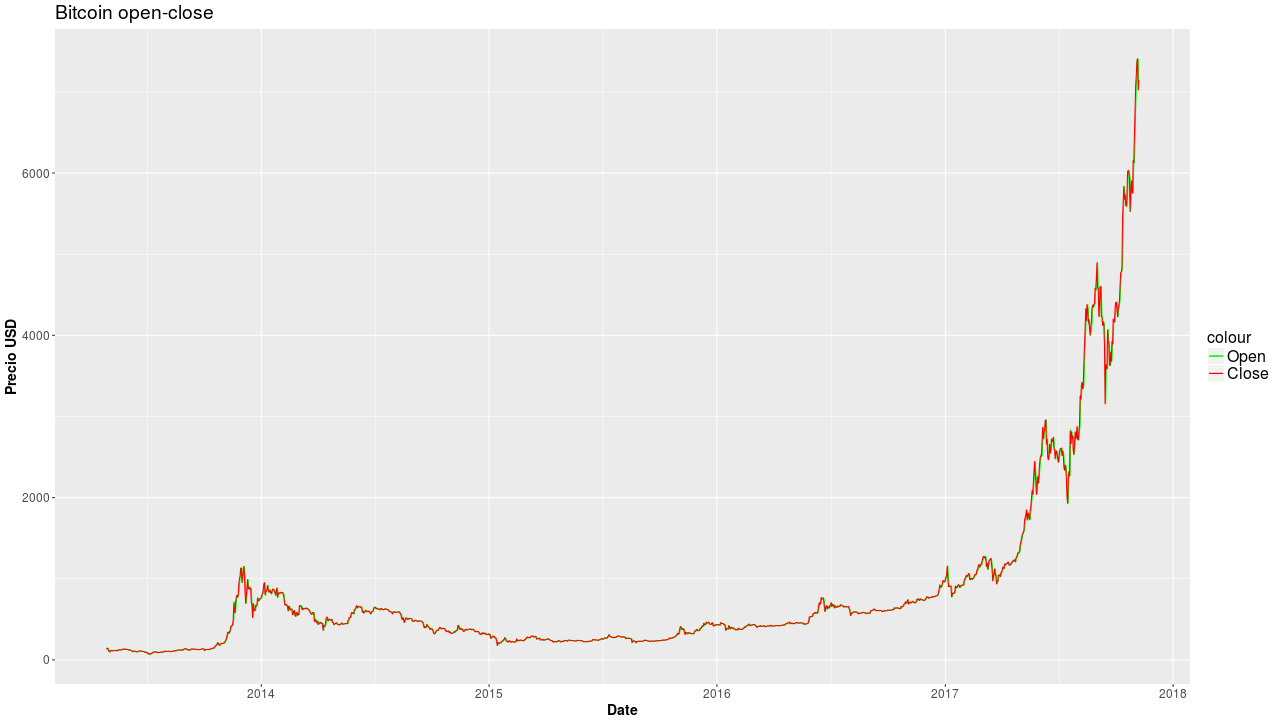
\includegraphics[width = 18cm, height = 10cm]{btc/date_vs_open-close}

        \caption{Precio en que abre y cierra btc}
    \end{figure}

    En realidad no se puede extrar mucha informaci\'on porque lo que se alcanza a visualizar esta encimado y no se aprecia un dato de otro. Entonces graficamos las diferencias, tal y como se muestra en la figura 2.

    \begin{figure}
        \centering

        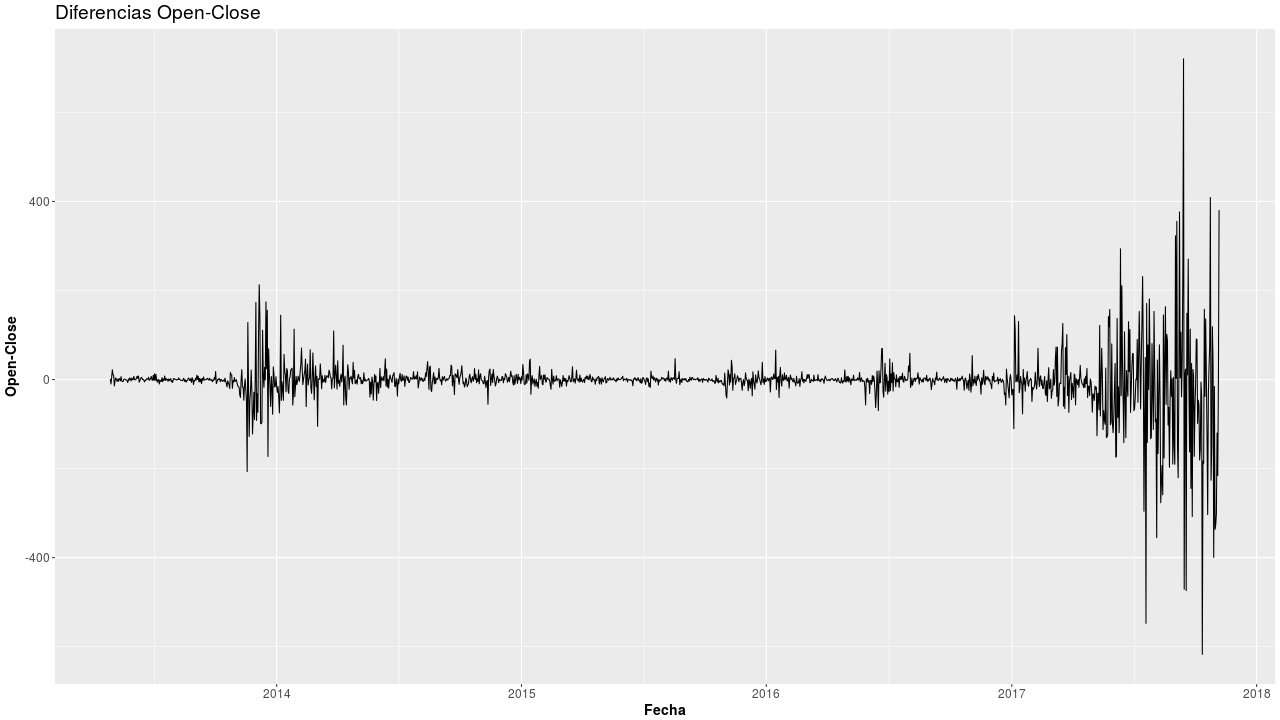
\includegraphics[width = 18cm, height = 10cm]{btc/diferencias_BTC_OpenClose}

        \caption{Diferencias de precio en que abre y cierra btc}
    \end{figure}

    Lo que se puede ver es que hay dos secciones con cambios muy abruptos: la primera es por 2013 y se puede ver que el precio lleg\'o a variar cerca de 400 dolares durante ese tiempo.
    \\
    La otra secci\'on es mucho m\'as actual, por los \'ultimos meses de 2017 y las variaciones en precio aqu\'i son m\'as pronunciadas, de cerca del doble que se ve en 2013.
    \\
    Comparado con esos dos puntos, la gr\'afica se comporta con relativamente poca volativilidad.
    \\
    Nos interes\'o ver con un poco m\'as de detalle las secciones de grandes cambios por lo que tambi\'en las graficamos con la esperanza de tener un mejor panorama. Estas se muestran en las figuras 3 y 4.
    
    \begin{figure}
        \centering

        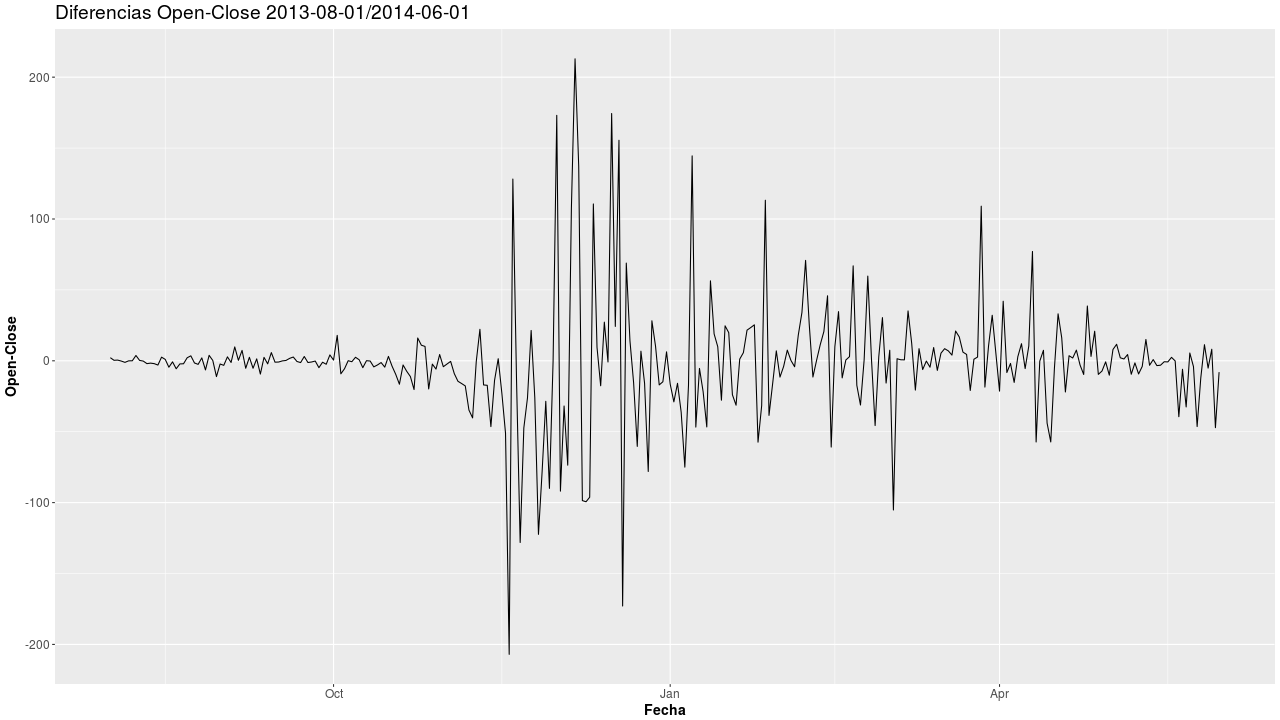
\includegraphics[width = 18cm, height = 10cm]{btc/diferencias_BTC_OpenClose_1}

        \caption{Diferencias de precio en que abre y cierra btc, acercamiento 2013} 
    \end{figure}

    \begin{figure}
        \centering

        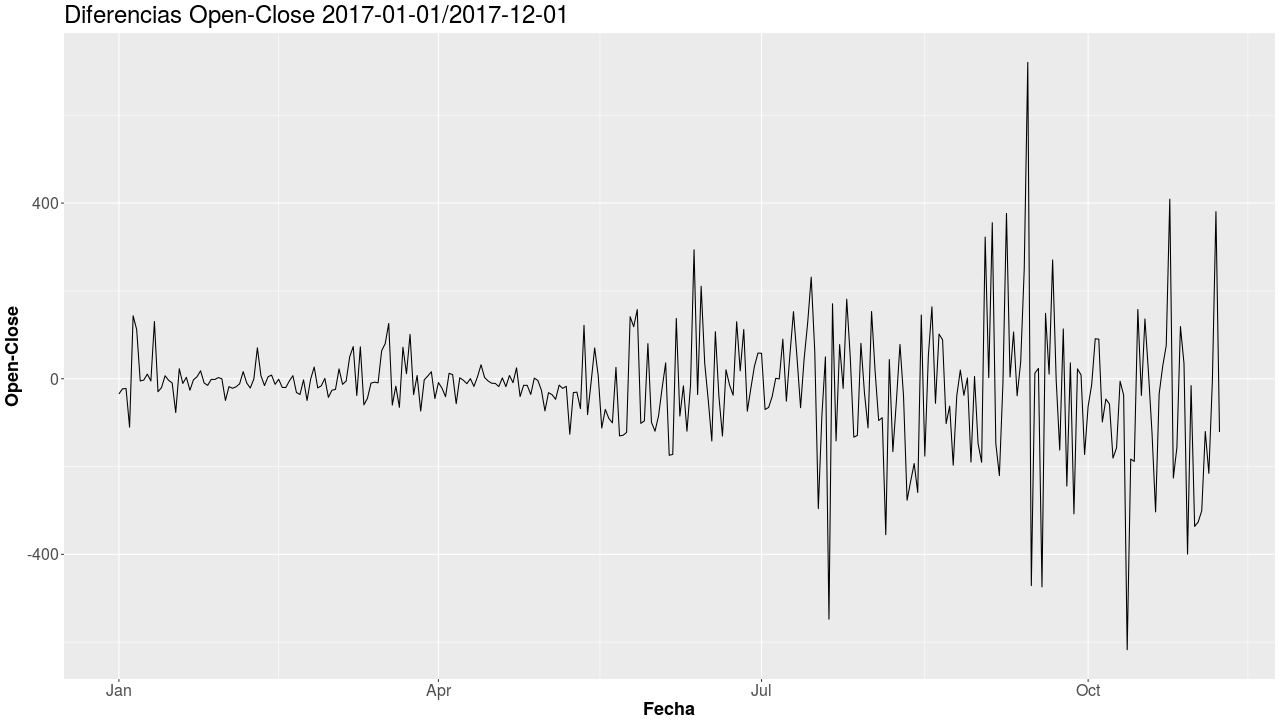
\includegraphics[width = 18cm, height = 10cm]{btc/diferencias_BTC_OpenClose_2}

        \caption{Diferencias de precio en que abre y cierra btc, acercamiento 2017}
    \end{figure}


    \begin{itemize}

        \item En general Los precios con los que abre la moneda se ven menores comparados con los que cierra.

        \item El caso de menor cambio en un d\'ia fue el 18 de Mayo de 2013 donde el Bitcoin cerro con el mismo precio que con el que abri\'o.

        \item El caso en el que en un d\'ia el precio del Bitcoin perdi\'o m\'as valor de inicio al fin fue el 14 de Septiembre de 2017 con una perdida de 720.42 dolares.

        \item El caso en el que en un d\'ia el precio del Bitcoin gan\'o m\'as valor de inicio al fin fue el 12 de Octubre de 2017 con una ganancia de 617.33 dolares.

    \end{itemize}


    \subsubsection*{Precio más alto y más bajo de un día}

    El precio m\'as alto o m\'as bajo de un d\'ia dice mucho sobre como fluctua el precio y por eso queremos analizarlo.
    \\

    En la siguiente figura se puede observar como han fluctuado el precio m\'as alto y bajo del Bitcoin en un d\'ia. Se puede observar que a diferencia de figura con de abertura y cierre, en esta los datos no estan completamente sobrepuestos y se puede notar, aunque pobremente muy pobremente, la diferencia entre el precio alto y el bajo.
    \\

    \begin{figure}
        \centering

        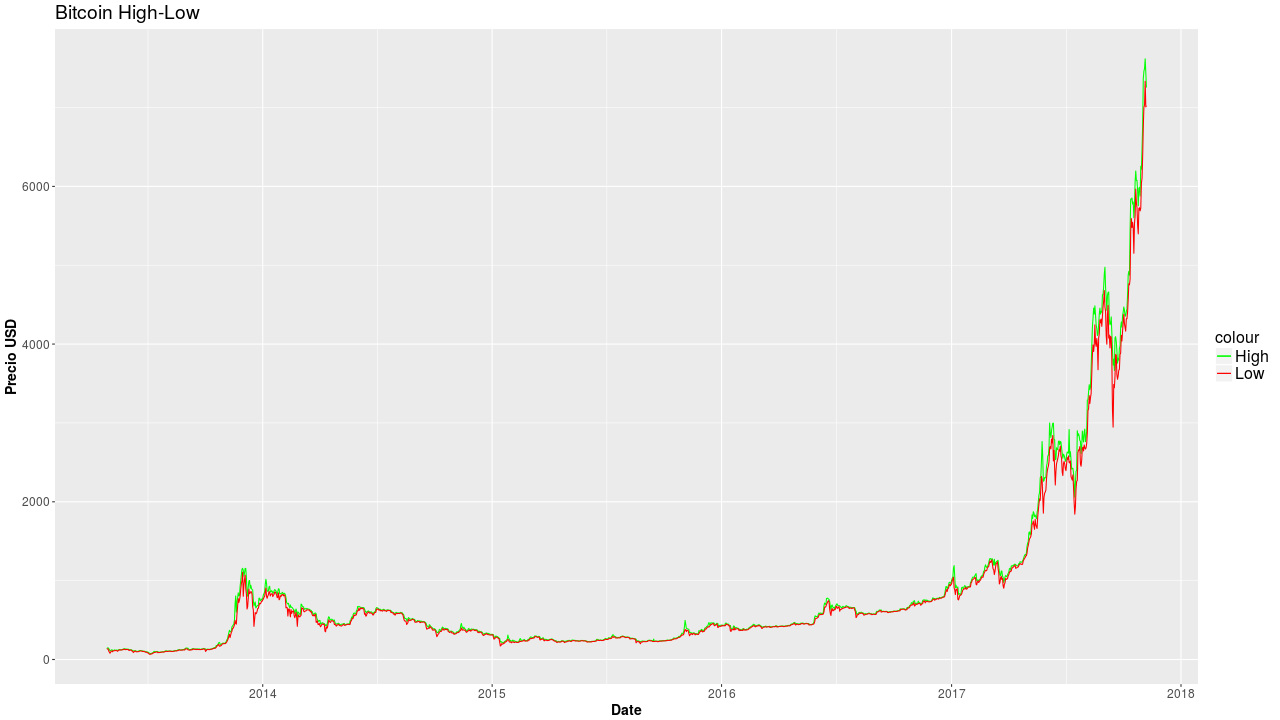
\includegraphics{btc/date_vs_high-low}

        \caption{Precio m\'as alto y m\'as bajo btc}
    \end{figure}

    En un esfuerzo para ver mejor las diferencias que hay, tambi\'en graficamos las diferencias y con esto quiza encontrar alg\'un patr\'on.

    \begin{figure}
        \centering

        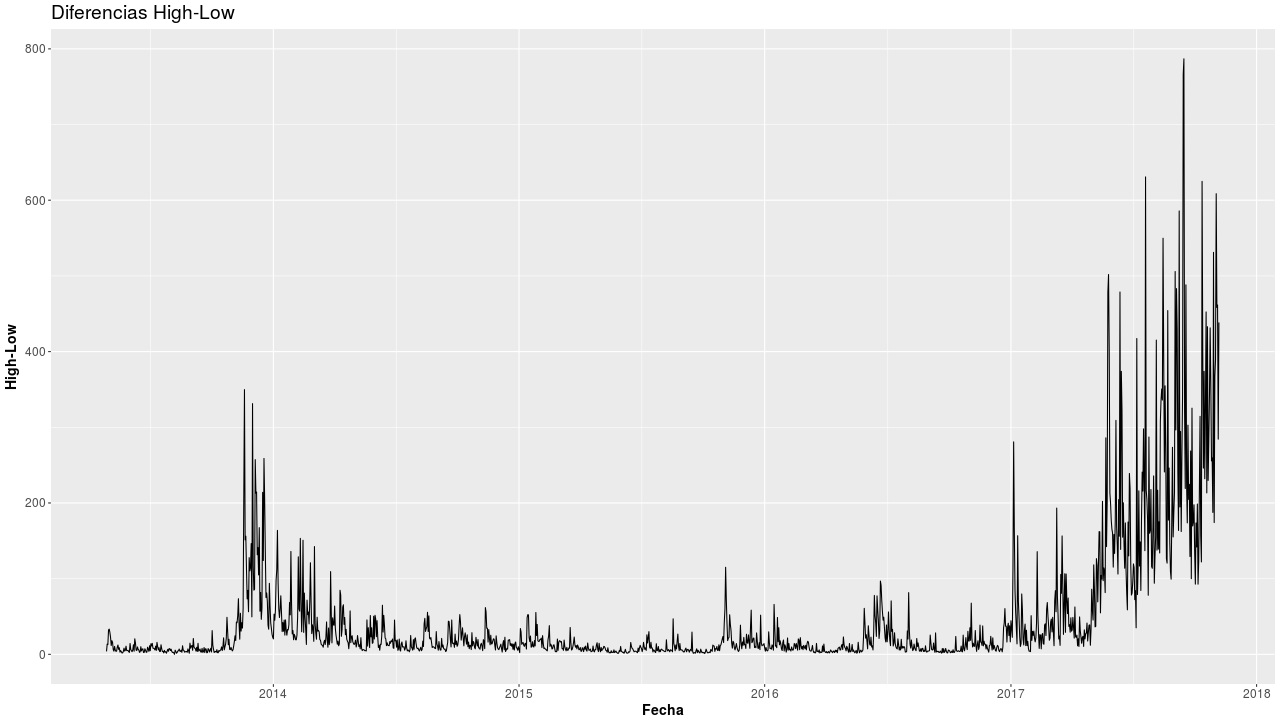
\includegraphics[width = 18cm, height = 10cm]{btc/diferencias_BTC_HighLow}

        \caption{Diferencias de precio m\'as alto y m\'as bajo btc}
    \end{figure}

    A finales de 2013 y principios del 2014 se ve bastante variaci\'on de los datos pero no se compara a la que se ve durante la segunda mitad del 2017. Hechamos un vistazo m\'as cercano a estos datos y vemos que las altas varianzas que se ve\'ian en 2013 fue cerca del final del a\~no en donde el llego a haber diferencia de m\'as de 300 dolares y en 2017 las diferencias de m\'as del doble de ese tiempo.

    \begin{figure}
        \centering

        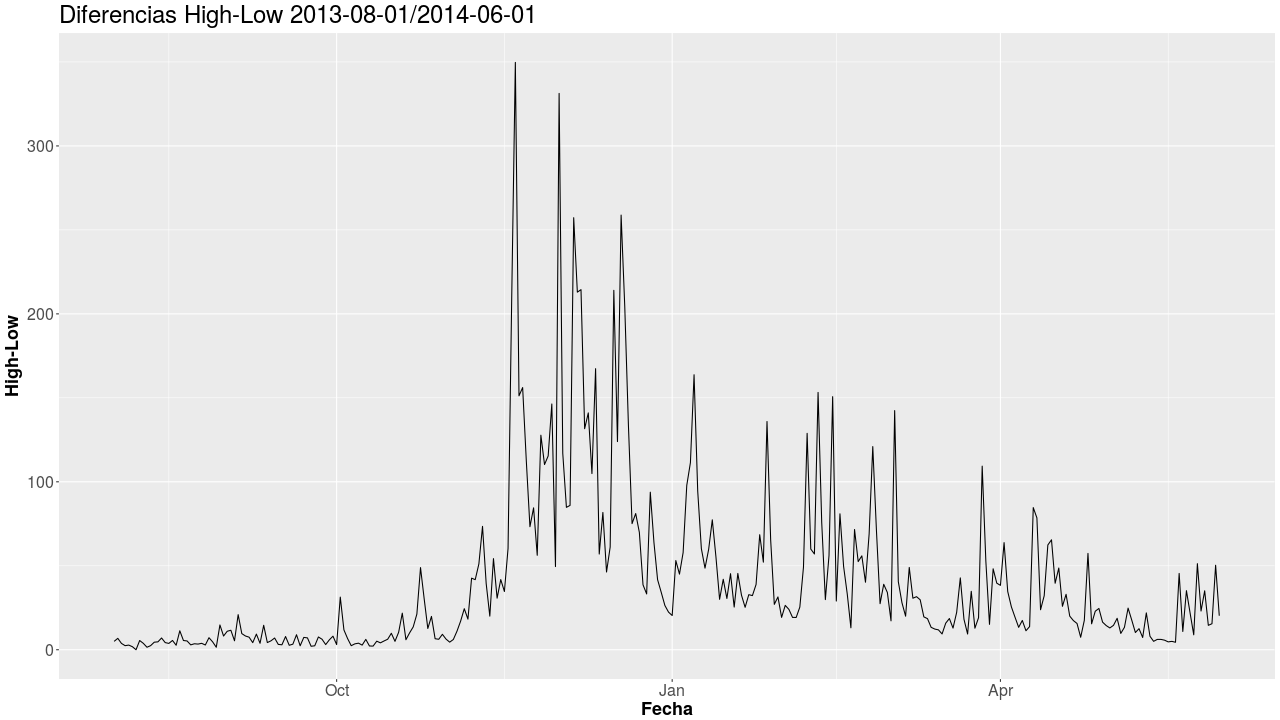
\includegraphics[width = 18cm, height = 10cm]{btc/diferencias_BTC_HighLow_1}

        \caption{Diferencias de precio m\'as alto y m\'as bajo btc, acercamiento 2013}
    \end{figure}

    \begin{figure}
        \centering

        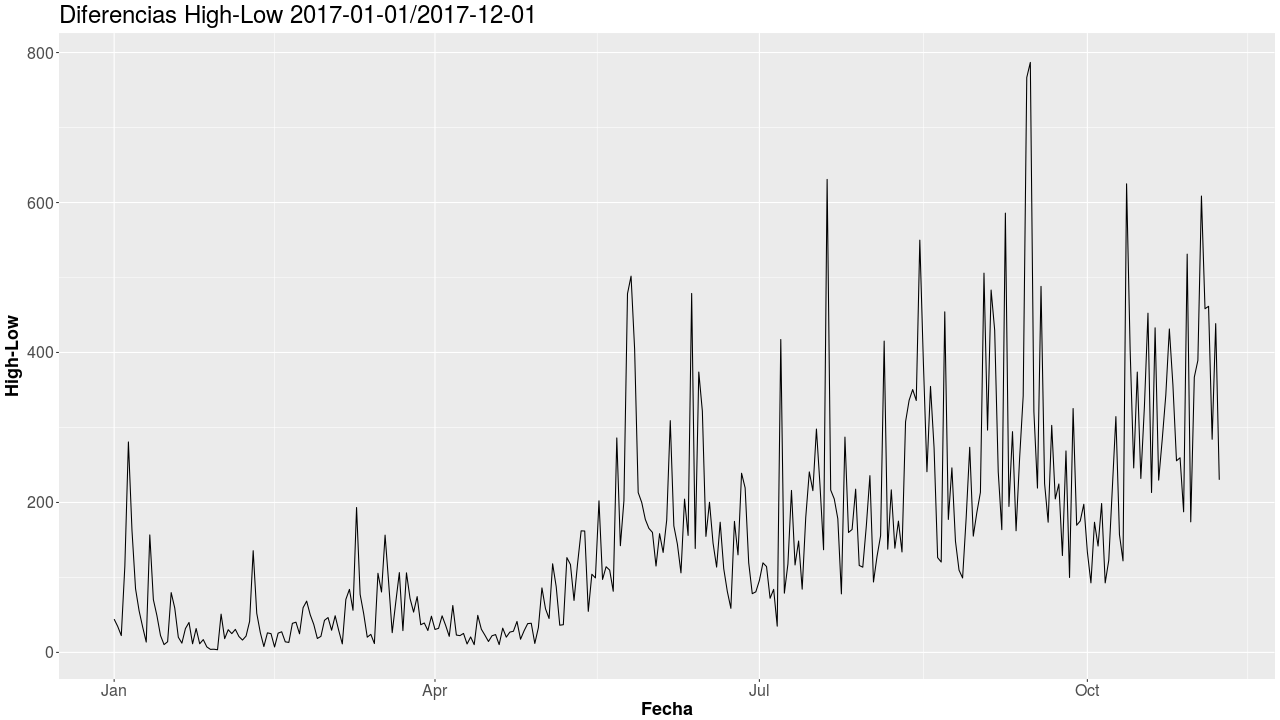
\includegraphics[width = 18cm, height = 10cm]{btc/diferencias_BTC_HighLow_2}

        \caption{Diferencias de precio m\'as alto y m\'as bajo btc, acercamiento 2017}
    \end{figure}


    \begin{itemize}

        \item El caso de menor cambio en un d\'ia fue el 18 de Mayo de 2013 donde el Bitcoin no cambi\'o de preci\'o ya que el valor m\'as alto y m\'as bajo de la moneda fue el mismo.

        \item El caso en el que en un d\'ia el precio del Bitcoin tuvo m\'as varianza fue el 15 de Septiembre de 2017 ya que la diferenc\'ia entre el valor m\'as alto y m\'as bajo es de 786.83 dolares.

        \item Es interesante como la fecha con menor variaci\'on de alto y bajo concuerda con la fecha de menor variaci\'on del precio en que abre y cierra y que el d\'ia de mayor variaci\'on de alto y bajo est\'a a solo un d\'ia del de abertura y cierre.

    \end{itemize}



    Por curiosidad, revisamos que tan seguido el precio máximo o mínimo era durante los periodos de apertura o cierre del día para las monedas.

    \begin{table}[h]
    \centering
    \caption{Relaci\'on de mayor o menor precio de acuerdo al principio, mitad o final del d\'ia}
    \label{label4}
    \begin{tabular}{|l|l|l|l|}
    \hline
    \rowcolor[HTML]{FFFFFF} 
    {\color[HTML]{333333} Bitcoin} & {\color[HTML]{333333} Abre} & {\color[HTML]{333333} Durante} & {\color[HTML]{333333} Cierra} \\ \hline
    Es mayor                       & 60                          & 1540                           & 55                            \\ \hline
    Es menor                       & 116                         & 1511                           & 28                            \\ \hline
    \end{tabular}
    \end{table}

    \begin{table}[h]
    \centering
    \caption{Relaci\'on de mayor o menor precio de acuerdo al principio, mitad o final del d\'ia}
    \label{label5}
    \begin{tabular}{|l|l|l|l|}
    \hline
    \rowcolor[HTML]{FFFFFF} 
    {\color[HTML]{333333} Ethereum} & {\color[HTML]{333333} Abre} & {\color[HTML]{333333} Durante} & {\color[HTML]{333333} Cierra} \\ \hline
    Mayor                           & 48                          & 745                            & 30                            \\ \hline
    Menor                           & 49                          & 752                            & 22                            \\ \hline
    \end{tabular}
    \end{table}

    \begin{table}[h]
    \centering
    \caption{Relaci\'on de mayor o menor precio de acuerdo al principio, mitad o final del d\'ia}
    \label{label6}
    \begin{tabular}{|l|l|l|l|}
    \hline
    \rowcolor[HTML]{FFFFFF}
    {\color[HTML]{333333} Bitcoin Cash} & {\color[HTML]{333333} Abre} & {\color[HTML]{333333} Durante} & {\color[HTML]{333333} Cierra} \\ \hline
    Mayor                               & 6                           & 101                            & 1                             \\ \hline
    Menor                               & 5                           & 96                             & 7                             \\ \hline
    \end{tabular}
    \end{table}

    Con esto encontramos:

    \begin{itemize}

        \item  Todos los porcentajes se mantienen por debajo del 10\% sin contar el durante.

        \begin{itemize}

            \item Para el Bitcoin, la más alta es la relaci\'on del precio de apertura con el precio más bajo en el día, 7\% de las veces con 116 días.
            
            \item El más bajo fue cuando el precio con el que cierra es el más bajo, con solo 1.7\% que fueron 28 días.

            \item Esto solo representa poco más del 15\% por lo que en su mayoría, los altos y los bajos de la moneda se daban no en el comienzo o final, si no durante el día.

        \end{itemize}

        \begin{itemize}

            \item Similarmente para Ethereum, la más alta es el precio de apertura con el precio más bajo en el día, 5.9\% de las veces con 49 días.
            
            \item El más bajo fue cuando el precio con el que cierra es el más bajo, con solo 2.7\% que fueron 22 días.

            \item Para el Ethereum, esto solo representa poco más del 18\% por lo que en su mayoría, los altos y los bajos de la moneda se daban no en el comienzo o final, si no durante el día.

        \end{itemize}

        \begin{itemize}

            \item Finalmente para Bitcoin cash, el valor más alto es un 6.5\%, que para Bitcoin cash son 7 días, en el precio más bajo es el que cierra.

            \item El porcentaje más bajo es de 0.92\% ,o un día, en el que el precio más alto es con el que se cierra.
    
            \item Para Bitcoin Cash, esto solo representa menos del 18\% por lo que en su mayoría, los altos y los bajos de la moneda se daban no en el comienzo o final, si no durante el día.
        \end{itemize}

    \end{itemize}


    \subsubsection*{¿Es el número de Bitcoins representado por una función geom\'etrica?}

    \begin{figure}
        \centering

        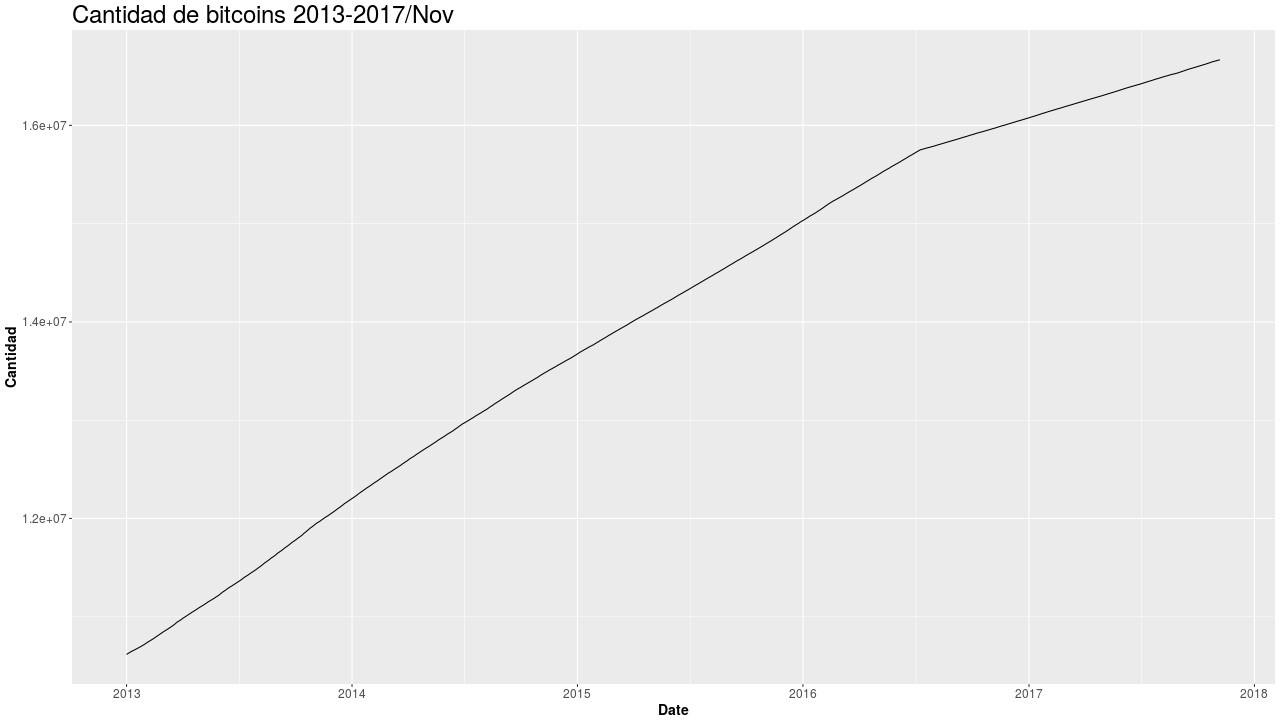
\includegraphics[width = 18cm, height = 10cm]{btc/fecha_vs_cantidad}

        \caption{Cantidad de Bitcoins a trav\'es del tiempo}
    \end{figure}

    Como se puede observar, el n\'umero de bitcoins es constante en intervalos de aproximadamente cuatro a\~nos y, despu\'es de ese periodo, se nota una disminuci\'on de pendiente, en el caso de la figura se pueden ver ya dos. Si siguiera con ese comportamiento de disminuci\'on de pendiente entonces llegar\'ia un punto en el que la pendiente ser\'ia 0. ¿Ser\'a ese el caso?, y si lo es, ¿Con cuantas monedas se dentendr\'ia?
    \\

    Ya se menciono con anterioridad que el n\'umero de Bitcoins m\'aximos es 21 millones. Esto se debe a que la funci\'on que decide cuantos Bitcoins se dan como recompensa es de una serie geom\'etrica y su l\'imite tiende a ese n\'umero, pero, ser\'a esto cierto? 

    Primero hay que ver a que se debe que digan que son 21 millones.
    \\

    \begin{enumerate}

        \item Bitcoin fue programado con la idea de que un nuevo bloque se descubre cada 10 minutos. Esto lo hace adaptivamente, es decir, aumenta o disminuye la dificultad de encontrar un nuevo bloque dependiendo de cuanto se tard\'o en encontrar el \'ultimo bloque.

        \item La recompensa por encontrar un bloque fue de inicialmente 50 Bitcoins.
            
        \item La recompensa por encontrar un bloque se divide en 2 cada <<ciclo>>, siendo un ciclo cada 4 a\~nos.

        \item Aunque no se sabe porque se eligieron estas constantes en particular, estos datos son suficientes para calcular el n\'umero m\'aximo de monedas.

    \end{enumerate}


    Consideremos lo siguiente: 
    \begin{itemize}
        \item 6 bloques por hora 

        \item 24 horas en un d\'ia

        \item 365 d\'ias en un a\~no

        \item4 a\~nos para un ciclo

    \end{itemize}

    $$6 * 24 * 365 * 4 = 210240$$

    $$210240 \approx 210000$$

    Estos son el n\'umero de bloques que son necesarios para que la recompensa sea reducida a la mitad.

    Para el n\'umero de bitcoins se tiene que encontrar el resultado de la suma infinita de monedas por bloques:
    
    $$ \sum_{i = 0}^{\infty} \frac{50}{2^{i}} = 50 + 25 + 12.5 + ...$$

    Esto es equivalente a la serie:

    $$ 50 \sum_{i = 0}^{\infty} \frac{1}{2^{i}} = 50 (1 + 0.5 + 0.25 + ...) $$

    Y la serie geom\'etrica resultante se sabe que es:

    $$ 50 \sum_{i = 0}^{\infty} \frac{1}{2^{i}} = 50 (2) $$

    $$ 50 \sum_{i = 0}^{\infty} \frac{1}{2^{i}} = 100 $$

    Con esto, solo es necesario multiplicar los resultados que obtuvimos:

    $$ 210000 * 100 = 21000000 $$

    Entonces, como ya no se conseguir\'an nuevos Bitcoins, ¿Ya no se crear\'an m\'as bloques?
    \\
    Este resultado no significa que ya no se a\~nadiran nuevos bloques al Blockchain una vez que se hayan minado todas las monedas, agregar bloques es necesario para el funcionamiento del protocolo, pero aunque se agreguen m\'as bloques, la recompenza de Bitcoins ser\'a de 0.
    \\

    Ya que conocemos la f\'ormula para generar el n\'umero de bloques, uno esperar\'ia poder predecir el n\'umero de mondeas en un cierto tiempo. Intentemos hacer eso:
    \\
    Considerando la fecha inicial, 3 de Enero de 2009, intentemos calcular cuantos bitcoins debe haber en ciertas fechas:
    \\
    En un a\~no se deber\'ian crear $6 * 24 * 365 * 50$ Bitcoins, estas son 2628000 monedas.
    \\
    En un a\~no y medio se deber\'ian crear $6 * 24 * 547 * 50$ Bitcoins, equivalente a 3938400 monedas.
    \\
    En 5 a\~nos se deber\'ian crear $(6 * 24 * 1460 * 50) + (6 * 24 * 365 * 25)$ Bitcoins, equivalente a 11826000 monedas.
    \\
    Pero cuando se revisa en los datos que se tienen se ve como no concuerdan:

    \begin{table}[h]
    \centering
    \caption{N\'umero de monedas que existen y que deber\'ian existir}
    \label{label7}
    \begin{tabular}{|l|l|l|l|l|}
    \hline
    \rowcolor[HTML]{FFFFFF}
    {\color[HTML]{333333} Fecha} & {\color[HTML]{333333} Total monedas  calculadas} & {\color[HTML]{333333} Total monedas existentes} & {\color[HTML]{333333} Error} & {\color[HTML]{333333} Error porcentual} \\ \hline
    2010-01-03                   & 2628000                                          & 1644000                                         & 0.3744                       & 37.44                                   \\ \hline
    2010-06-04                   & 3938400                                          & 2967250                                         & .2466                        & 24.66                                   \\ \hline
    2014-01-03                   & 11826000                                         & 12211525                                        & .0326                        & 3.26                                    \\ \hline
    \end{tabular}
    \end{table}

    Con estos pocos ejemplos podemos ver que hay discrepancias pronuciadas entre el n\'umero de Bitcoins calculados que deber\'ian haber y el que en realidad hay, ¿A que se puede deber esto?
    \\
    Cuando hicimos las predicciones del n\'umero de Bitcoins, estabamos asumiendo el caso que el programa considera optimo: que se agregar 6 bloques por hora, que desde el inicio se empezo con el ideal de n\'umero de bloques por hora y que los cambios en el poder de computo y la dificultad se cancelan el uno al otro todo el tiempo, las cuales son muy poco probables que hayan sucedido.

    Con esto que tenemos, veamos como se relacionan las monedas si el sistema funcionara de manera ideal y como realmente funciona:

    \begin{figure}
        \centering

        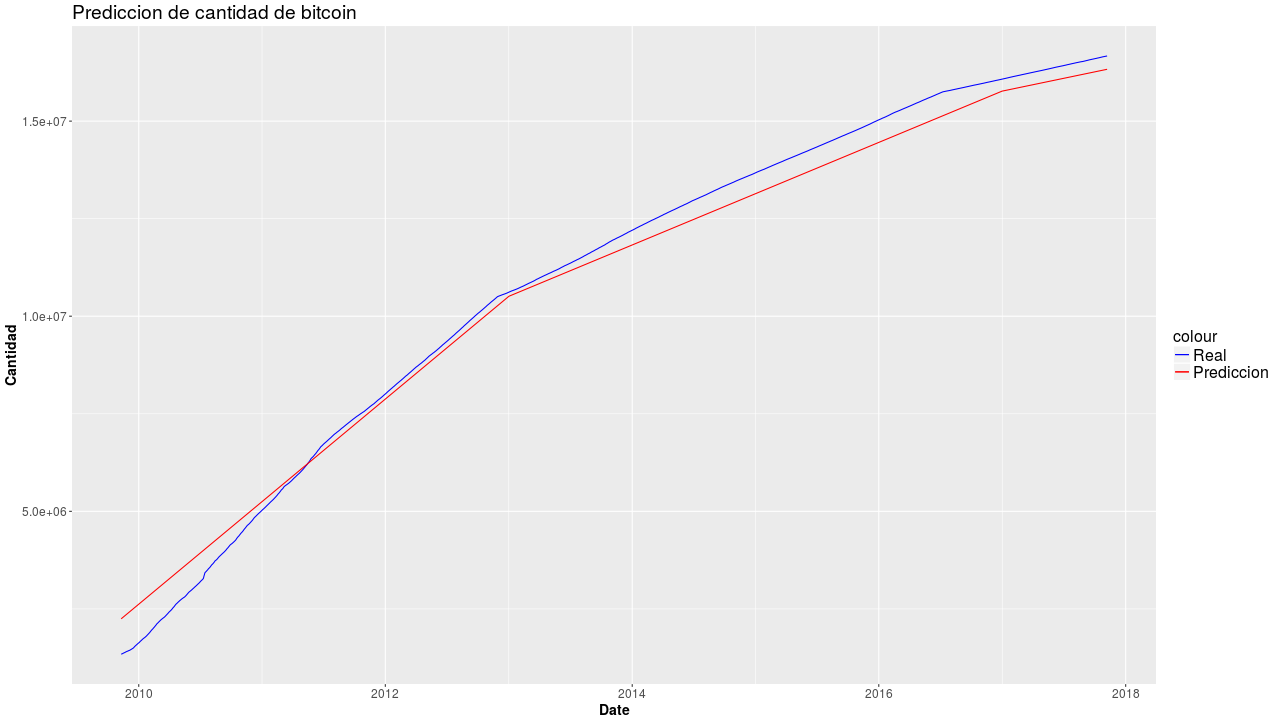
\includegraphics[width = 18cm, height = 10cm]{btc/prediccionBTC}

        \caption{N\'umero de Bitcoins y n\'umero de Bitcoins que deber\'ian existir}
    \end{figure}

    A simple vista las graficas se ven muy similares. Haremos una prueba de correlaci\'on para saber que tan relacionados est\'an los datos.
    \\
    La prueba pearson de correlaci\'on arroja como resultado un p-valor de $2.2e-16$, un intervalo de confianza de $(0.9988955, 0.9990446)$ con un nivel de confianza del 95\%. Ya que el p-valor obtenido es menor a 0.05, se puede concluir que la correlaci\'on entre los dos datos es significante.
    \\


    \subsubsection*{Cantidad de monedas y precio}

    Con un poco de conocimiento de economía, resulta natural pensar en relacionar la cantidad de monedas en un mercado con el precio que estas tienen. Entonces es de interes revisar si las criptomonedas cumplen con esto, es decir, si se puede ver dependencia entre la cantidad de criptomonedas y su precio.

    \begin{figure}
        \centering

        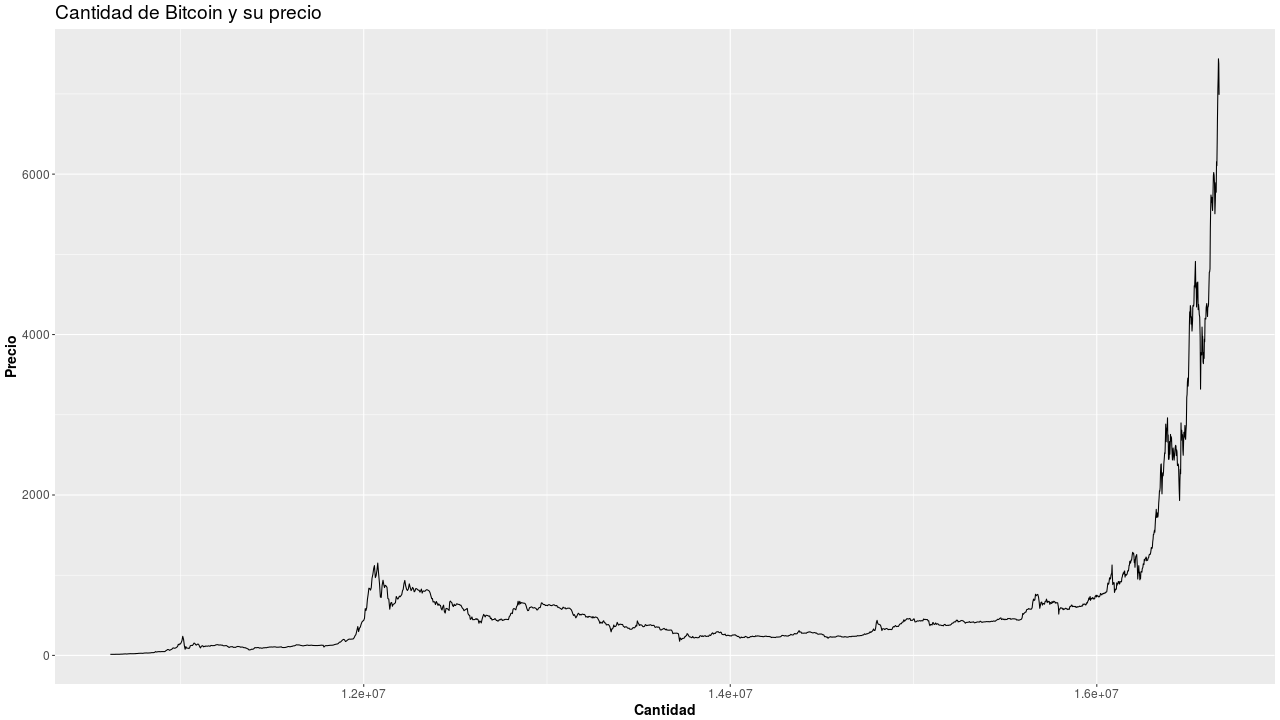
\includegraphics[width = 18cm, height = 10cm]{btc/cantidad_vs_precio}

        \caption{Cantidad de monedas contra precio de moneda}
    \end{figure}

    \subsubsection*{Blockchain}

    Como fue discutido al inicio, el protocolo Blockchain es lo que permitio que las criptomonedas existieran por haber solucionado el problema del gasto doble por lo que es de especial interes analizarlo al menos un poco, especificamente el tamaño del Blockchain ya que es uno de los datos que se tienen.

    Revisaremos si el tamaño del Blockchain y la cantidad de bitcoins estan correlacionados y si aumenta o disminuye con el tiempo.

    \begin{figure}
        \centering

        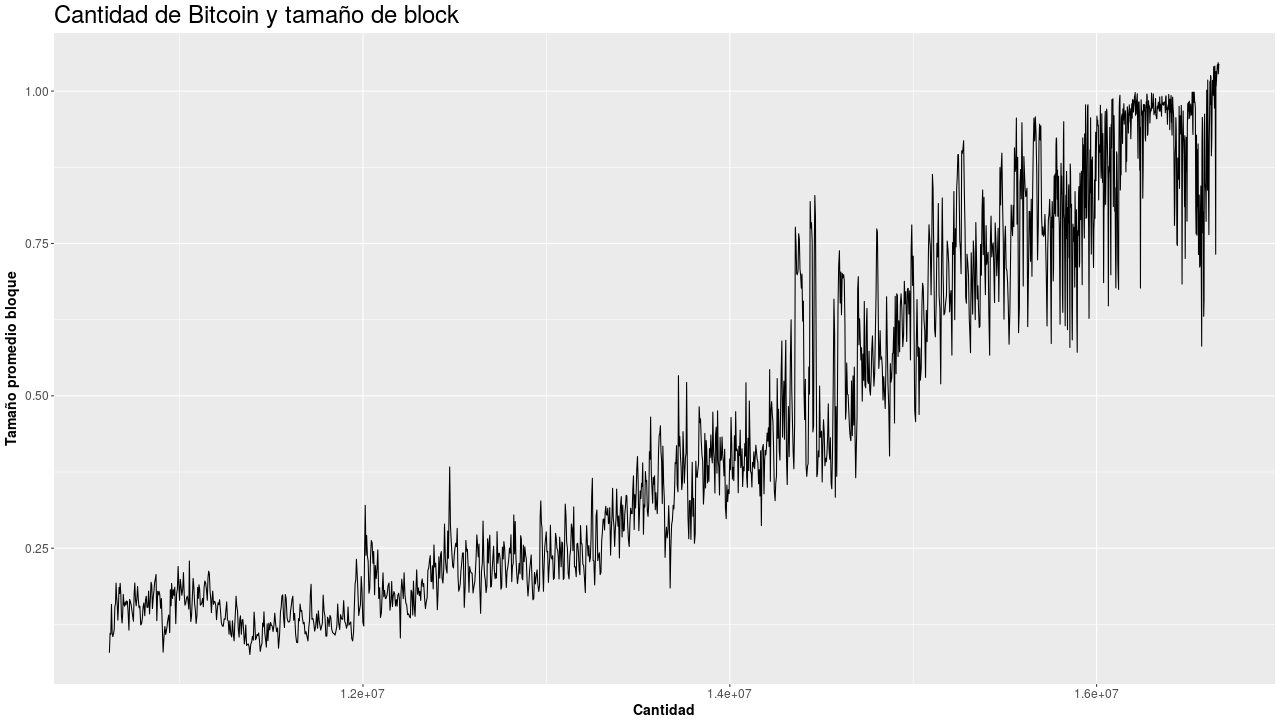
\includegraphics[width = 18cm, height = 10cm]{btc/blockSize_vs_cantidad}

        \caption{Tama\~no promedio de Blockchain contra cantidad de Bitcoins}
    \end{figure}

    \subsubsection*{Hash rate}

    Hash rate (o taza de hasheo) se refiere a que tan poderosa puede ser una maquina de un minero de criptomonedas, especificamente se refiere al número de veces que una función hash es calculada por segundo. Las ganancias que un minero espera son directamente proporcionales al hash rate.

    El como se relaciona el hash rate con el tiempo puede ser de interes porque se podria ver como avanza el número de calculos que los mineros deben de realizar con las monedas a través del tiempo.

    \begin{figure}
        \centering

        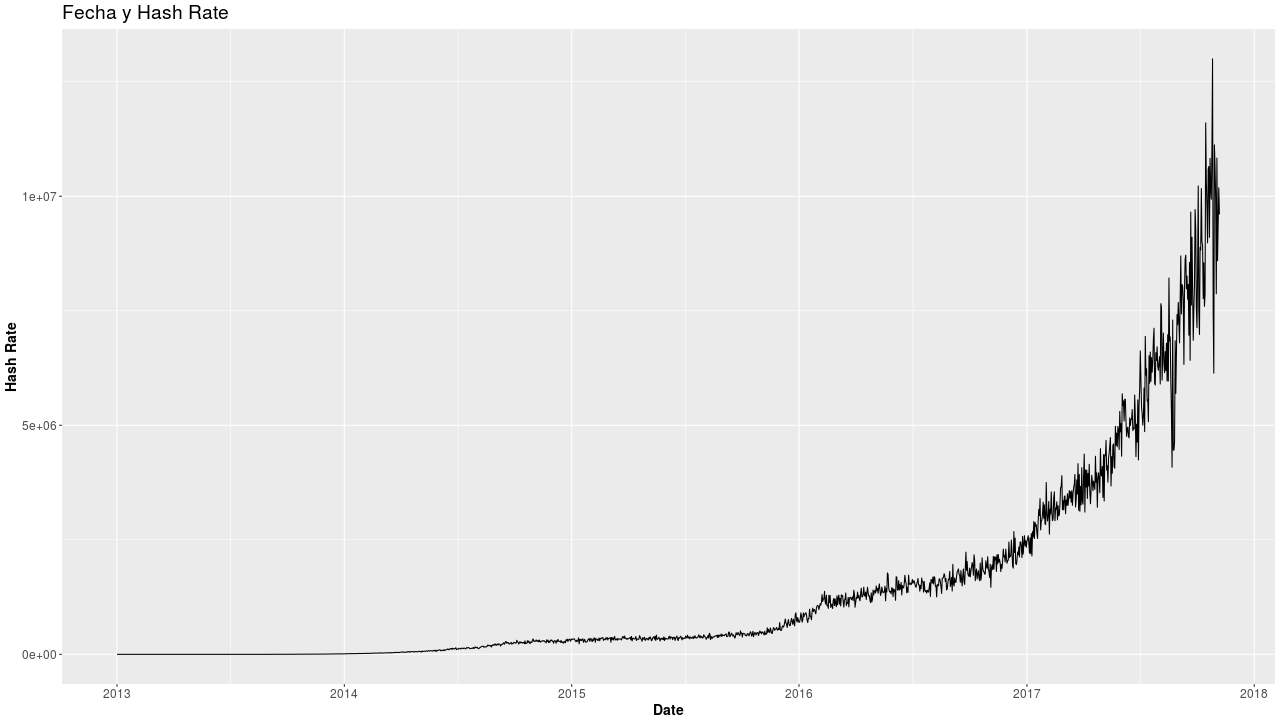
\includegraphics[width = 18cm, height = 10cm]{btc/date_vs_hashRate}

        \caption{Hash rate contra tiempo}
    \end{figure}

\section{Conclusiones}

	\subsubsection*{C\'omo es que el precio historico de las diferentes criptomonedas cambia en el tiempo?}
	\subsubsection*{Las criptomonedas son volatiles o estables?}
	\subsubsection*{Se relaciona la fluctiaci\'on de precio de una criptomoneda con otra?}
	\subsubsection*{Los cambios de precio se dan con respecto a temporadas?}

	
\section{Bibliografia}

\end{document}
